\documentclass[conference]{IEEEtran}
\IEEEoverridecommandlockouts
% The preceding line is only needed to identify funding in the first footnote. If that is unneeded, please comment it out.
%Template version as of 6/27/2024

\usepackage{cite}
\usepackage{amsmath,amssymb,amsfonts}
\usepackage{algorithmic}
\usepackage{graphicx}
\usepackage{float}
\usepackage{textcomp}
\usepackage{xcolor}

\def\BibTeX{{\rm B\kern-.05em{\sc i\kern-.025em b}\kern-.08em
    T\kern-.1667em\lower.7ex\hbox{E}\kern-.125emX}}
\begin{document}

\title{Conference Paper Title*\\
{\footnotesize \textsuperscript{*}Note: Sub-titles are not captured for https://ieeexplore.ieee.org  and
should not be used}
\thanks{Identify applicable funding agency here. If none, delete this.}
}

\author{\IEEEauthorblockN{1\textsuperscript{st} Given Name Surname}
\IEEEauthorblockA{\textit{dept. name of organization (of Aff.)} \\
\textit{name of organization (of Aff.)}\\
City, Country \\
email address or ORCID}
\and
\IEEEauthorblockN{2\textsuperscript{nd} Given Name Surname}
\IEEEauthorblockA{\textit{dept. name of organization (of Aff.)} \\
\textit{name of organization (of Aff.)}\\
City, Country \\
email address or ORCID}
\and
\IEEEauthorblockN{3\textsuperscript{rd} Given Name Surname}
\IEEEauthorblockA{\textit{dept. name of organization (of Aff.)} \\
\textit{name of organization (of Aff.)}\\
City, Country \\
email address or ORCID}
\and
\IEEEauthorblockN{4\textsuperscript{th} Given Name Surname}
\IEEEauthorblockA{\textit{dept. name of organization (of Aff.)} \\
\textit{name of organization (of Aff.)}\\
City, Country \\
email address or ORCID}
\and
\IEEEauthorblockN{5\textsuperscript{th} Given Name Surname}
\IEEEauthorblockA{\textit{dept. name of organization (of Aff.)} \\
\textit{name of organization (of Aff.)}\\
City, Country \\
email address or ORCID}
\and
\IEEEauthorblockN{6\textsuperscript{th} Given Name Surname}
\IEEEauthorblockA{\textit{dept. name of organization (of Aff.)} \\
\textit{name of organization (of Aff.)}\\
City, Country \\
email address or ORCID}
}

\maketitle

\begin{abstract}
This document is a model and instructions for \LaTeX.
This and the IEEEtran.cls file define the components of your paper [title, text, heads, etc.]. *CRITICAL: Do Not Use Symbols, Special Characters, Footnotes, 
or Math in Paper Title or Abstract.
\end{abstract}

\begin{IEEEkeywords}
component, formatting, style, styling, insert.
\end{IEEEkeywords}


\section{Resultados}
\subsection{Estrutura dos dados e checagens iniciais}

Durante o preprocessamento, verificamos que os dados não continham valores ausentes, mas uma presença considerável de outliers. Os intervalos e valores observados para as variáveis estavam dentro do esperado fisiologicamente. A frequência cardíaca variou aproximadamente dentro da faixa adulta típica (cerca de 50–180 bpm entre os indivíduos), com médias em torno de valores normais em repouso ($\approx$ 60-80 bpm) e elevações compatíveis com situações de maior demanda experimental.

A presença do atributo condition permitiu comparar os grupos, mas as médias não seguiram o padrão fisiológico clássico (HR maior e HRV menor em estresse), indicando que as classes representam indivíduos diferentes e não medições repetidas. Ainda assim, a Figura \ref{fig:kde_hr_rmssd} evidencia o comportamento global das variáveis entre condições.

\begin{figure}[H]
    \centering
    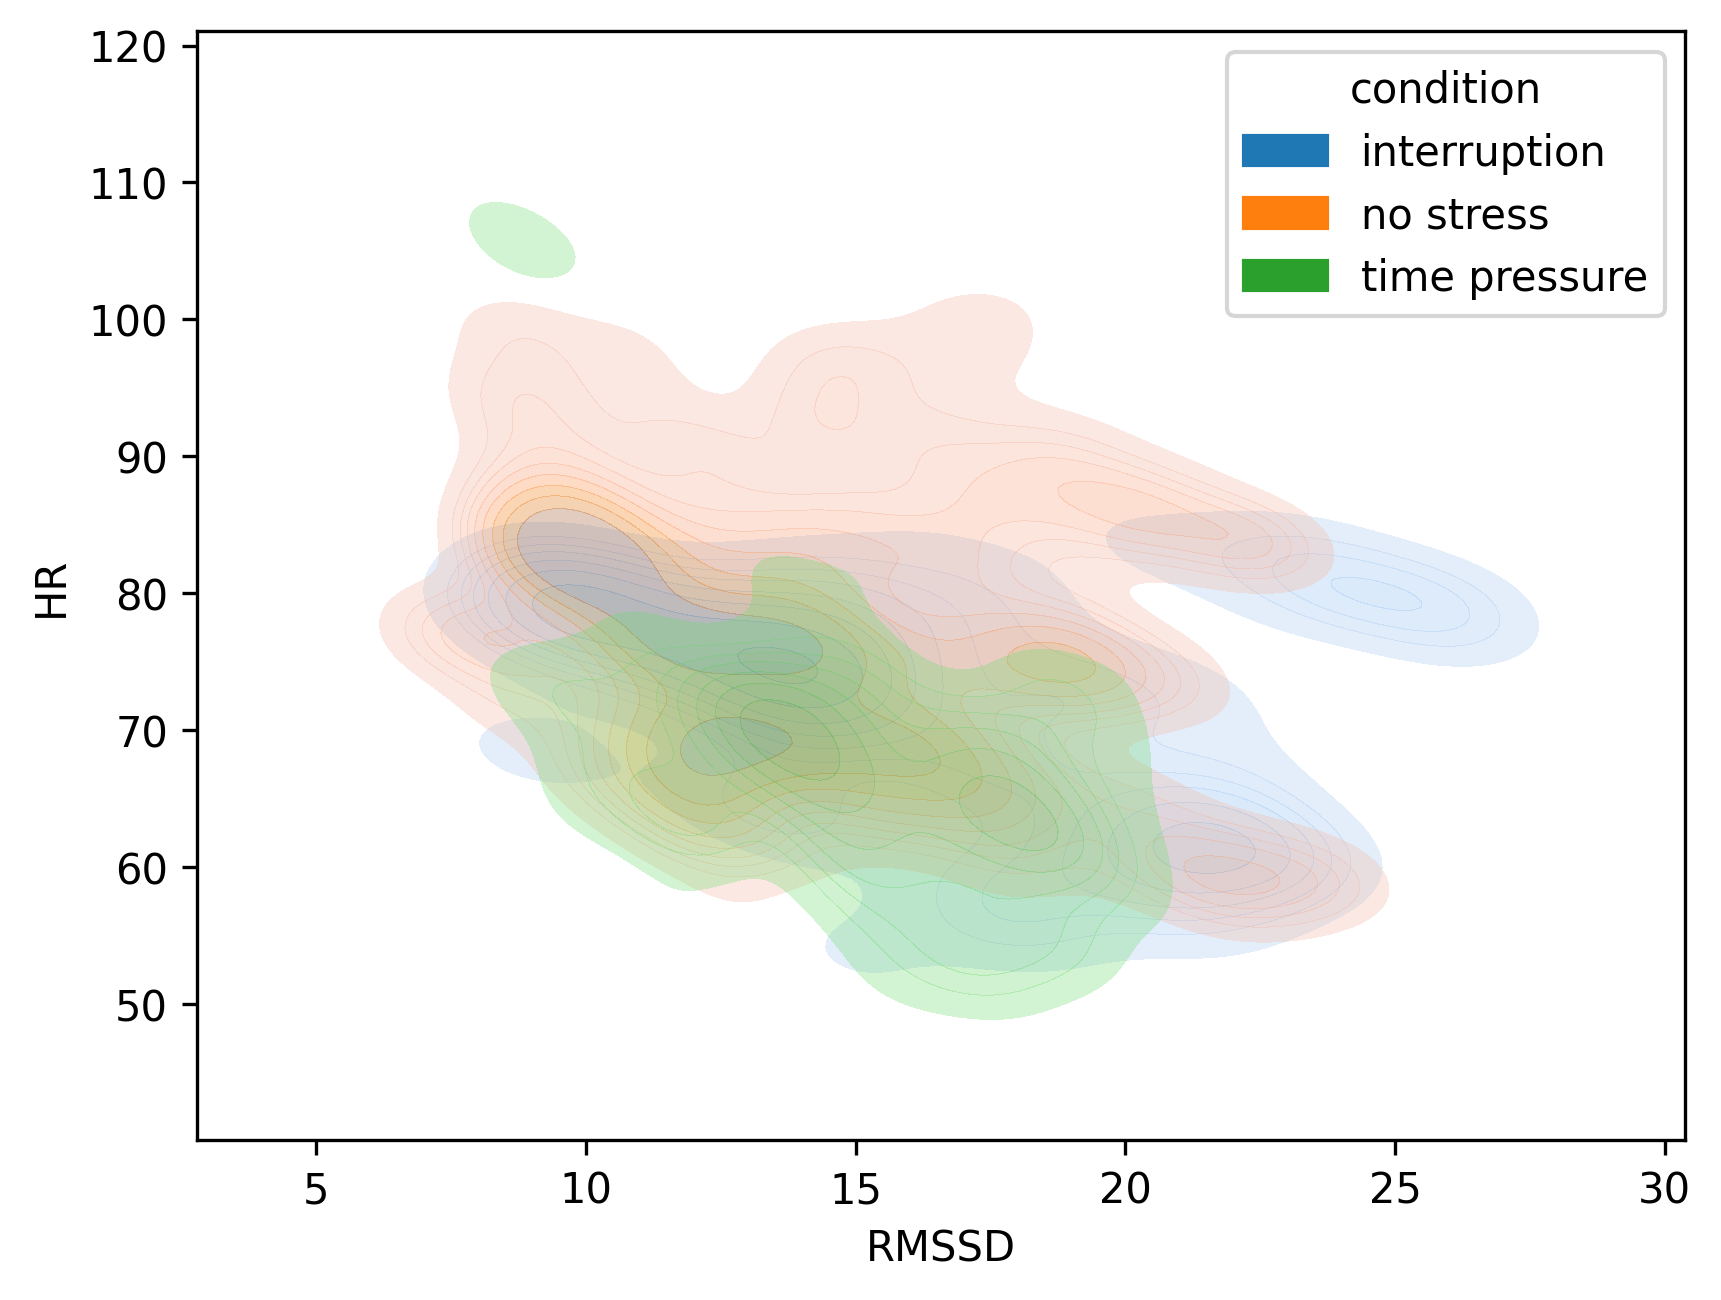
\includegraphics[width=0.7\linewidth]{../../../images/Anderson/kde_hr_rmssd_condition.png}
    \caption{Densidade bivariada HR × RMSSD nas diferentes condições.}
    \label{fig:kde_hr_rmssd}
\end{figure}

\subsection{Achados principais}

Após o pré-processamento e análise exploratória dos dados, identificamos padrões que relacionam as métricas de variabilidade da frequência cardíaca (HRV) com a frequência cardíaca medida (HR).

\subsubsection{Relação entre MEAN\_RR, MEDIAN\_RR e HR}

Inicialmente, há uma correlação inversa entre o intervalo R-R médio (MEAN\_RR) e a frequência cardíaca (HR), como na Figura \ref{fig:hr_median_rr}, indicando que intervalos menores entre batimentos estão associados a HR mais alta. O que é esperado, pois quanto menor o RR, maior o número de batimentos por minuto \cite{R1}.

Em repouso o RR costuma ser $\approx1$ segundo (HR $\approx60$ bpm), enquanto RR de 0,5 s implica HR $\approx120$ bpm (taquicardia). Em que, considera-se taquicardia um ritmo cardíaco de repouso acima de 100 bpm \cite{R2}, valor este que de fato foi ultrapassado em alguns registros do conjunto de dados, sugerindo episódios de estresse ou esforço significativos.

\begin{figure}[H]
    \centering
    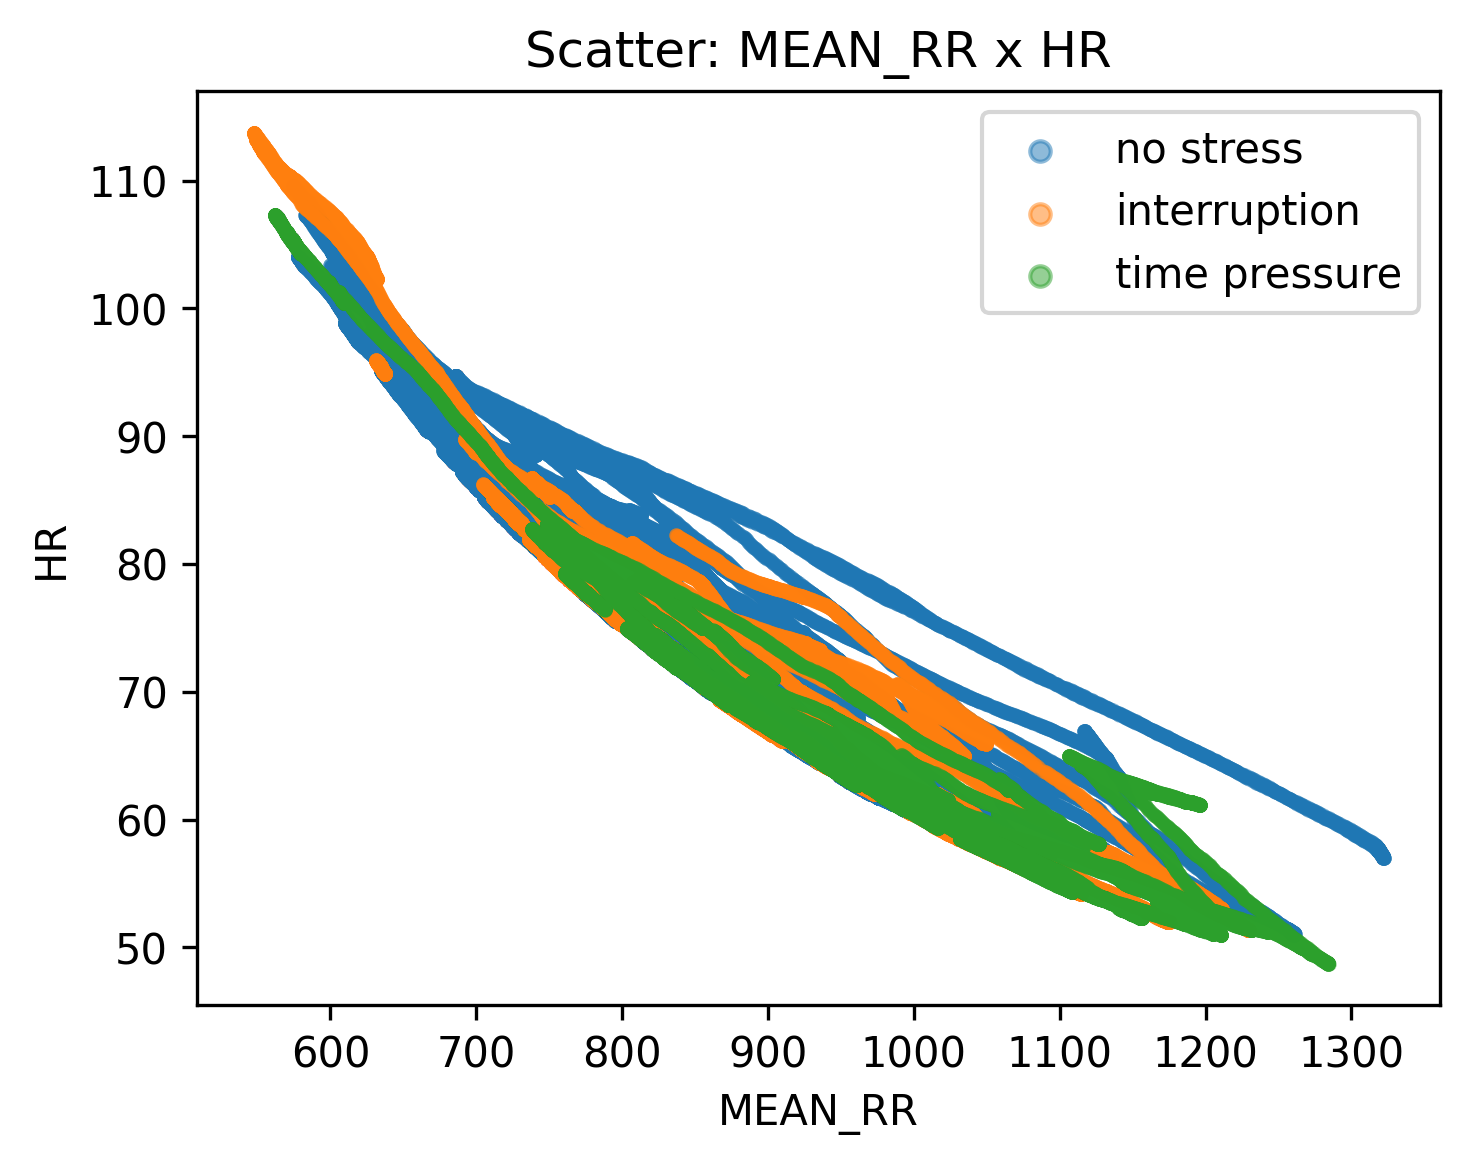
\includegraphics[width=0.8\linewidth]{../../../images/Anderson/Scatter_Condicional/Scatter MEAN_RR x HR.png}
    \caption{Dispersão HR × MEDIAN\_RR por classe}
    \label{fig:hr_median_rr}
\end{figure}

A mesma correlação forte e negativa ocorre entre MEDIAN\_RR e HR ($r\approx -0,93$). O que é esperado por definição, já que MEDIAN\_RR e MEAN\_RR carregam essencialmente a mesma informação fisiológica da frequência cardíaca, sendo altamente correlacionados, como representado na Figura \ref{fig:mean_median_rr}.

\begin{figure}[H]
    \centering
    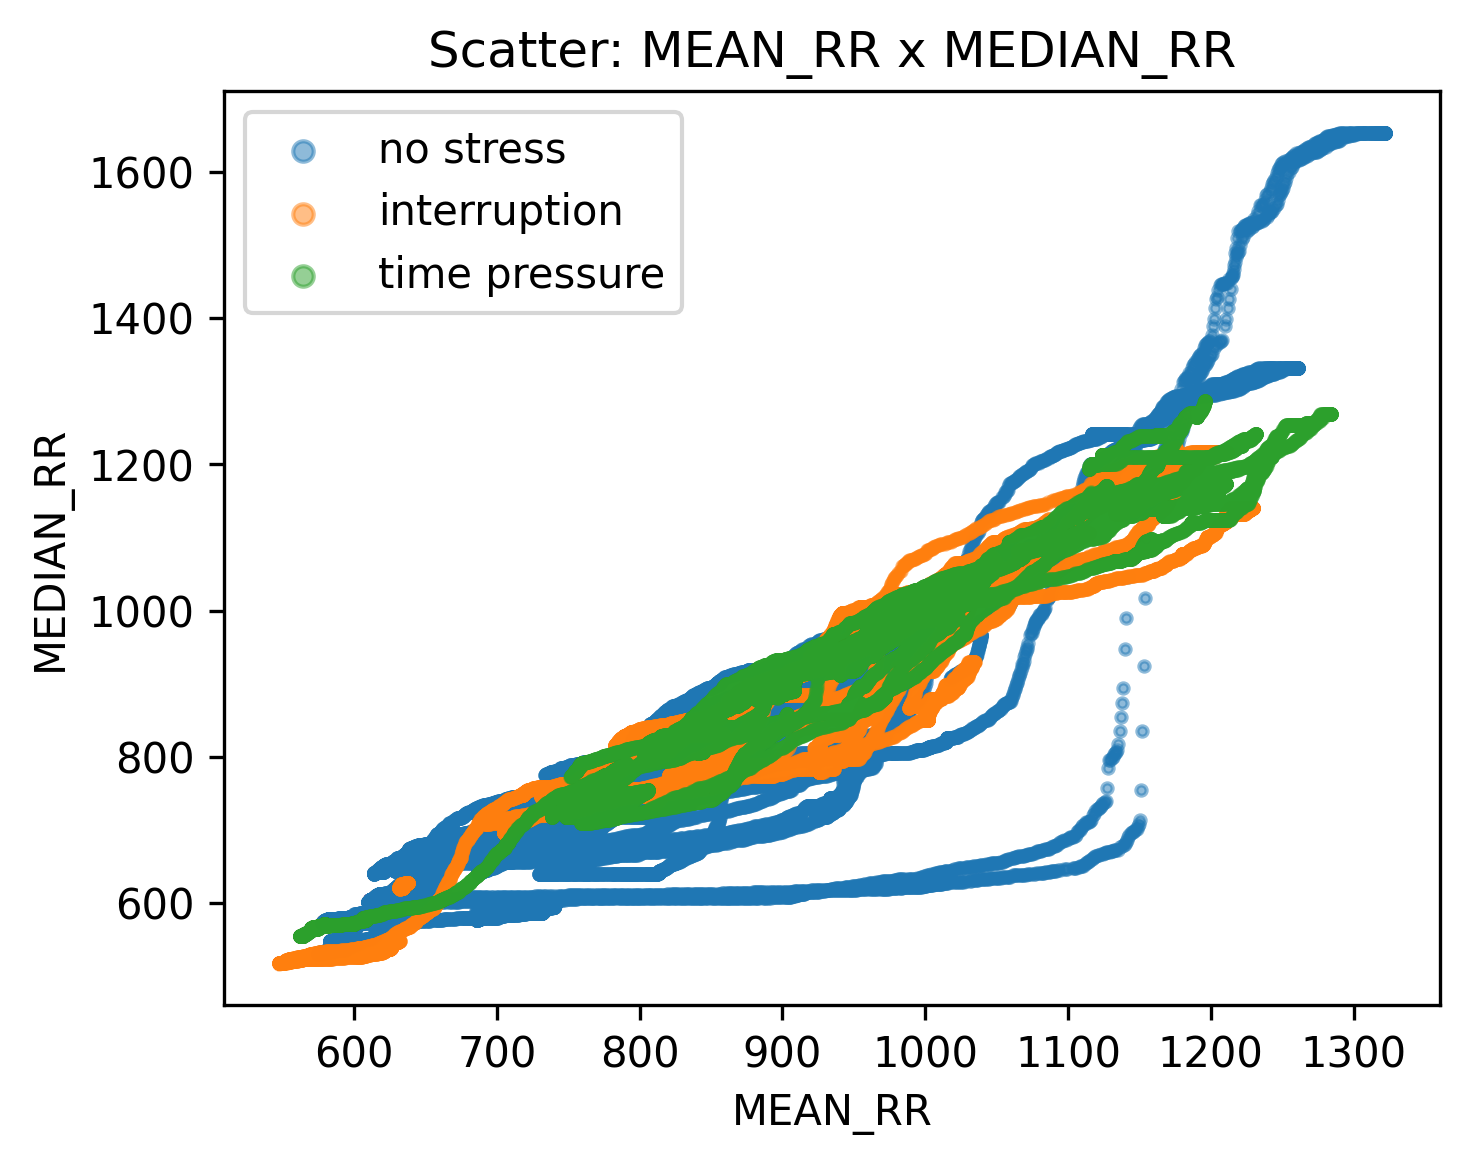
\includegraphics[width=0.8\linewidth]{../../../images/Anderson/Scatter_Condicional/Scatter MEAN_RR x MEDIAN_RR.png}
    \caption{Dispersão MEAN\_RR × MEDIAN\_RR por classe}
    \label{fig:mean_median_rr}
\end{figure}

\subsubsection{Variabilidade de curto e longo prazo}

Observamos que métricas clássicas de variabilidade, especialmente aquelas dominadas pelo tônus parassimpático, tendem a diminuir quando a frequência cardíaca está elevada. Por exemplo, indicadores como RMSSD (raiz quadrada da média dos quadrados das diferenças sucessivas de RR) e pNN50 (porcentagem de intervalos RR sucessivos que diferem em mais de 50ms) exibiram valores menores em casos de HR alto. O que sugerem menor variabilidade batimento a batimento durante episódios de frequência elevada, coincidindo com o esperado em situações de estresse ou ativação simpática.

Na literatura, condições de estresse psicológico costumam se associar a HRV reduzida, incluindo queda em métricas como pNN50 e potência de alta frequência (HF), indicando menor influência vagal, ao mesmo tempo em que a razão LF/HF se eleva \cite{R1}. Nossos dados seguem esse padrão geral: as condições associadas a maior demanda apresentaram pNN50 e RMSSD mais baixos e LF/HF mais altos, refletindo um desequilíbrio autonômico compatível com a ativação simpática (Figura \ref{fig:pnn50_X_LFHF}). Essa combinação de menor variabilidade de curto prazo e aumento relativo das oscilações de longo prazo sugere menor flexibilidade autonômica sob estresse, em consonância com o descrito na literatura \cite{R1}.

\begin{figure}[H]
    \centering
    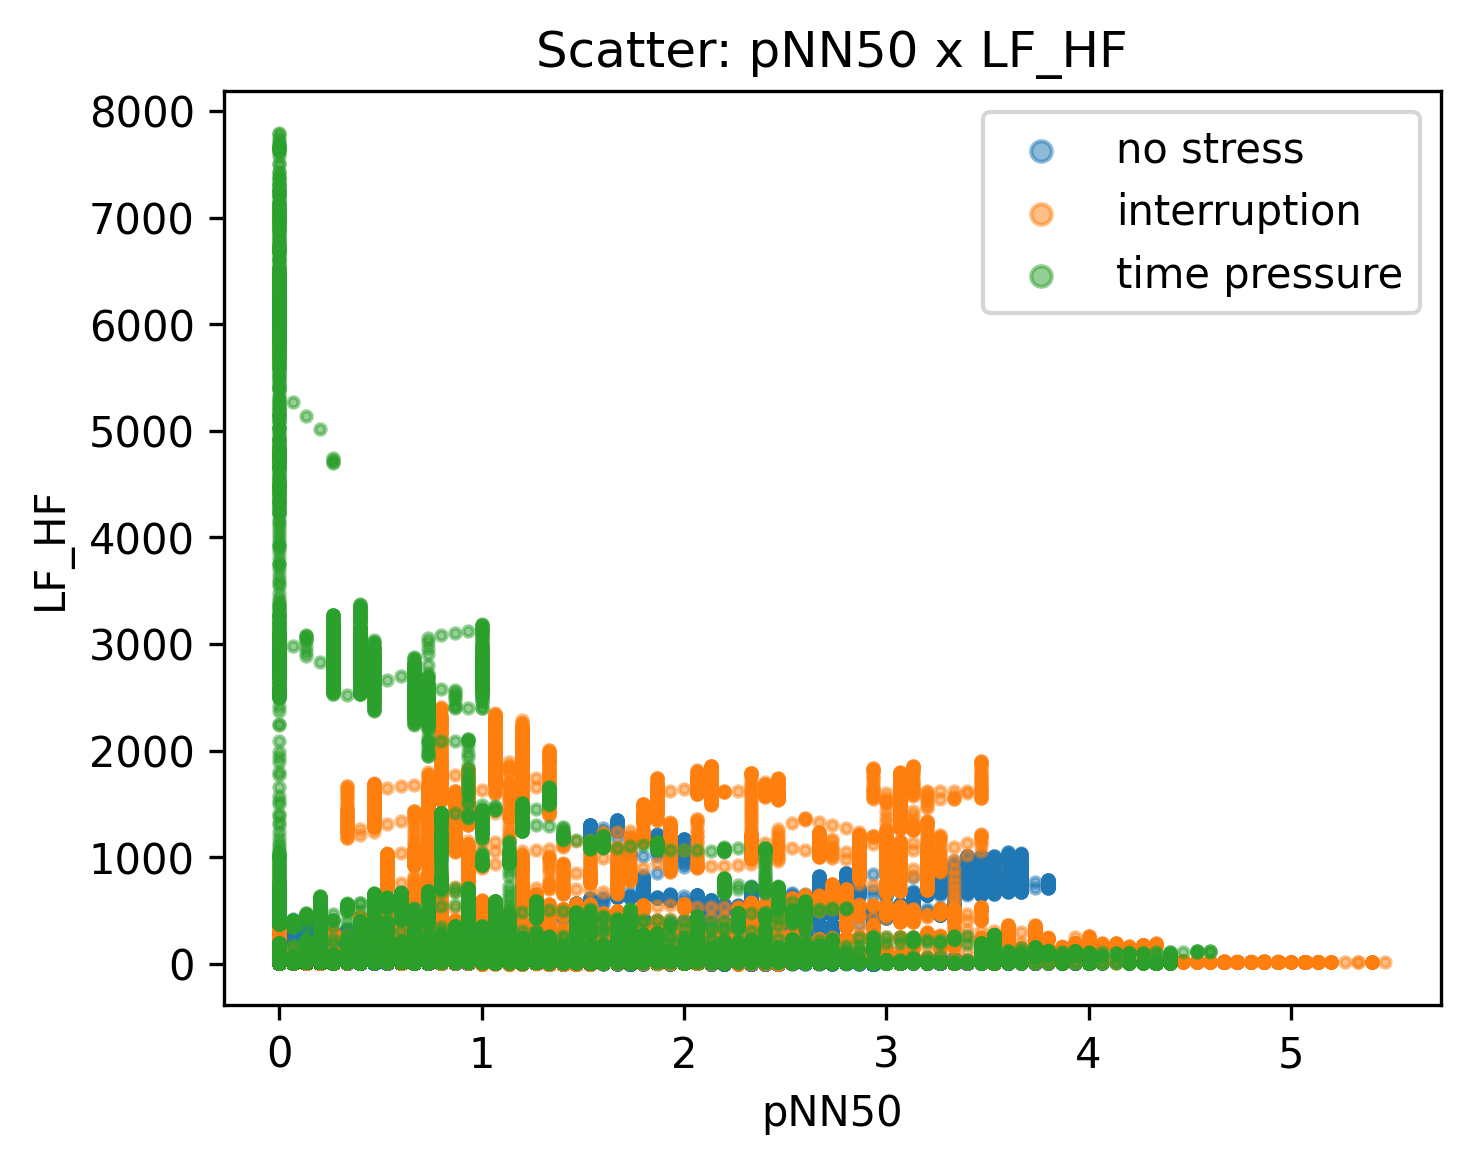
\includegraphics[width=0.8\linewidth]{../../../images/Anderson/Scatter_Condicional/Scatter pNN50 x LF_HF.png}
    \caption{Dispersão pNN50 × LF/HF por condição.}
    \label{fig:pnn50_X_LFHF}
\end{figure}

\subsubsection{Espectro e razão}

No domínio da frequência, vimos que, à medida que aumentava a demanda das tarefas (no stress $\rightarrow$ interruption $\rightarrow$ time pressure), a potência na banda de alta frequência (HF, 0,15–0,4 Hz) tendia a diminuir, enquanto a potência de baixa frequência (LF, 0,04–0,15 Hz) mostrava aumento relativo, resultando em elevação da razão LF/HF (Figura~\ref{fig:lfhf_box}). Esse comportamento indica uma redução da modulação vagal e maior predominância simpática, conforme descrito em estudos sobre respostas autonômicas ao estresse \cite{R1}.

As três condições do conjunto de dados apresentaram essa tendência de aumento progressivo da razão LF/HF, embora com grande dispersão. 

\begin{figure}[H]
    \centering
    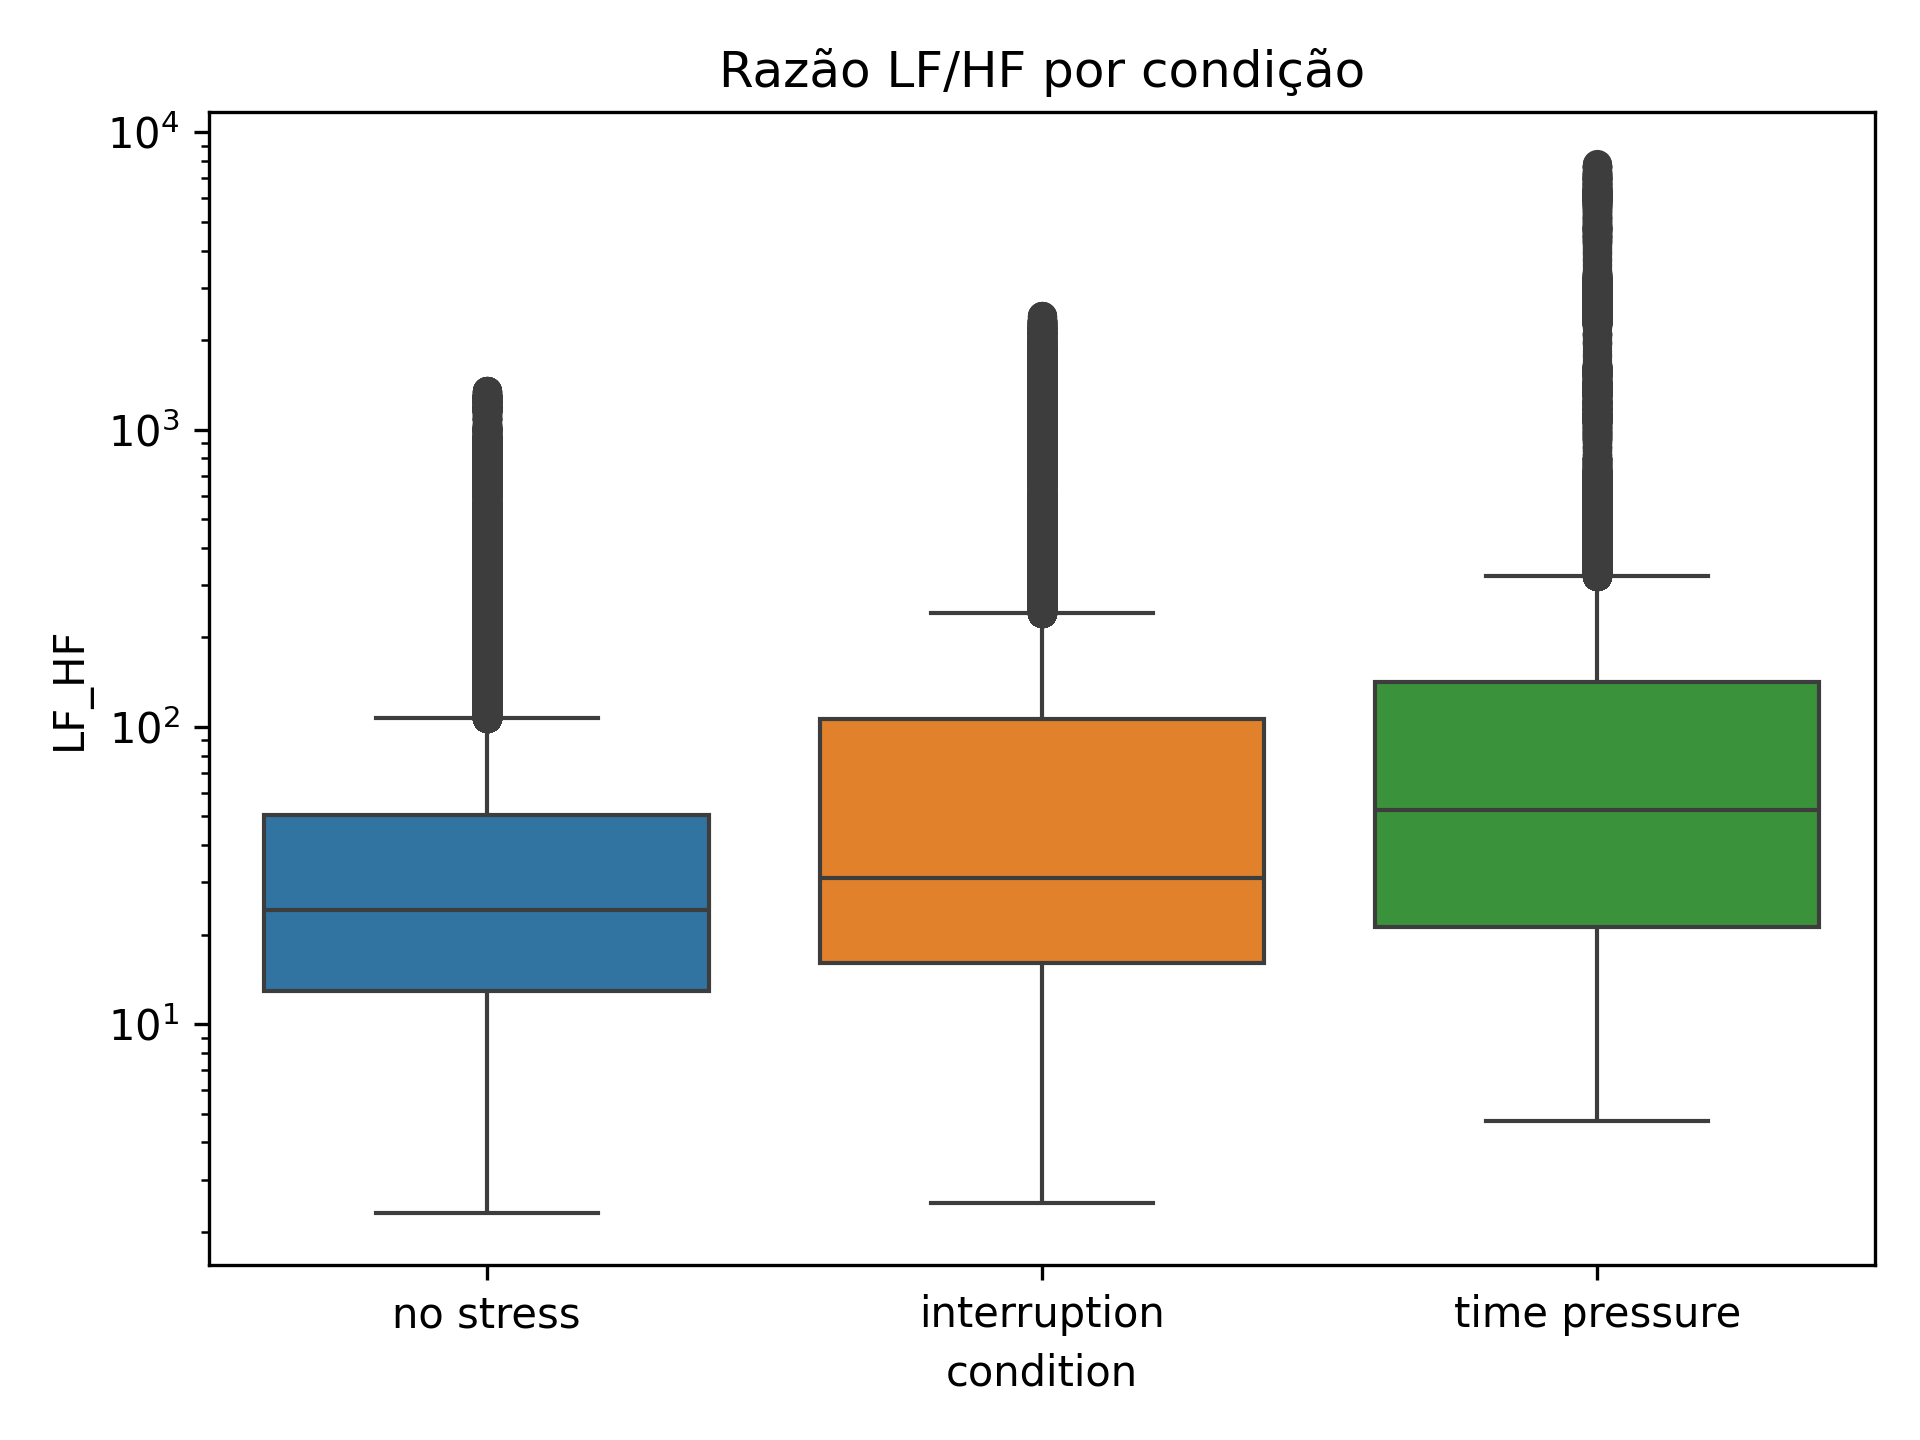
\includegraphics[width=0.8\linewidth]{../../../images/Anderson/box_lf_hf_condition.png}
    \caption{Boxplot LF/HF por condição.}
    \label{fig:lfhf_box}
\end{figure}

Quando a razão inversa (HF/LF) é observada, a interpretação se mantém invertida: em situações de maior demanda (menor influência vagal), HF diminui e LF aumenta, levando a LF/HF mais altos e, portanto, HF/LF mais baixos (Figura~\ref{fig:hflf_box}).

\begin{figure}[H]
    \centering
    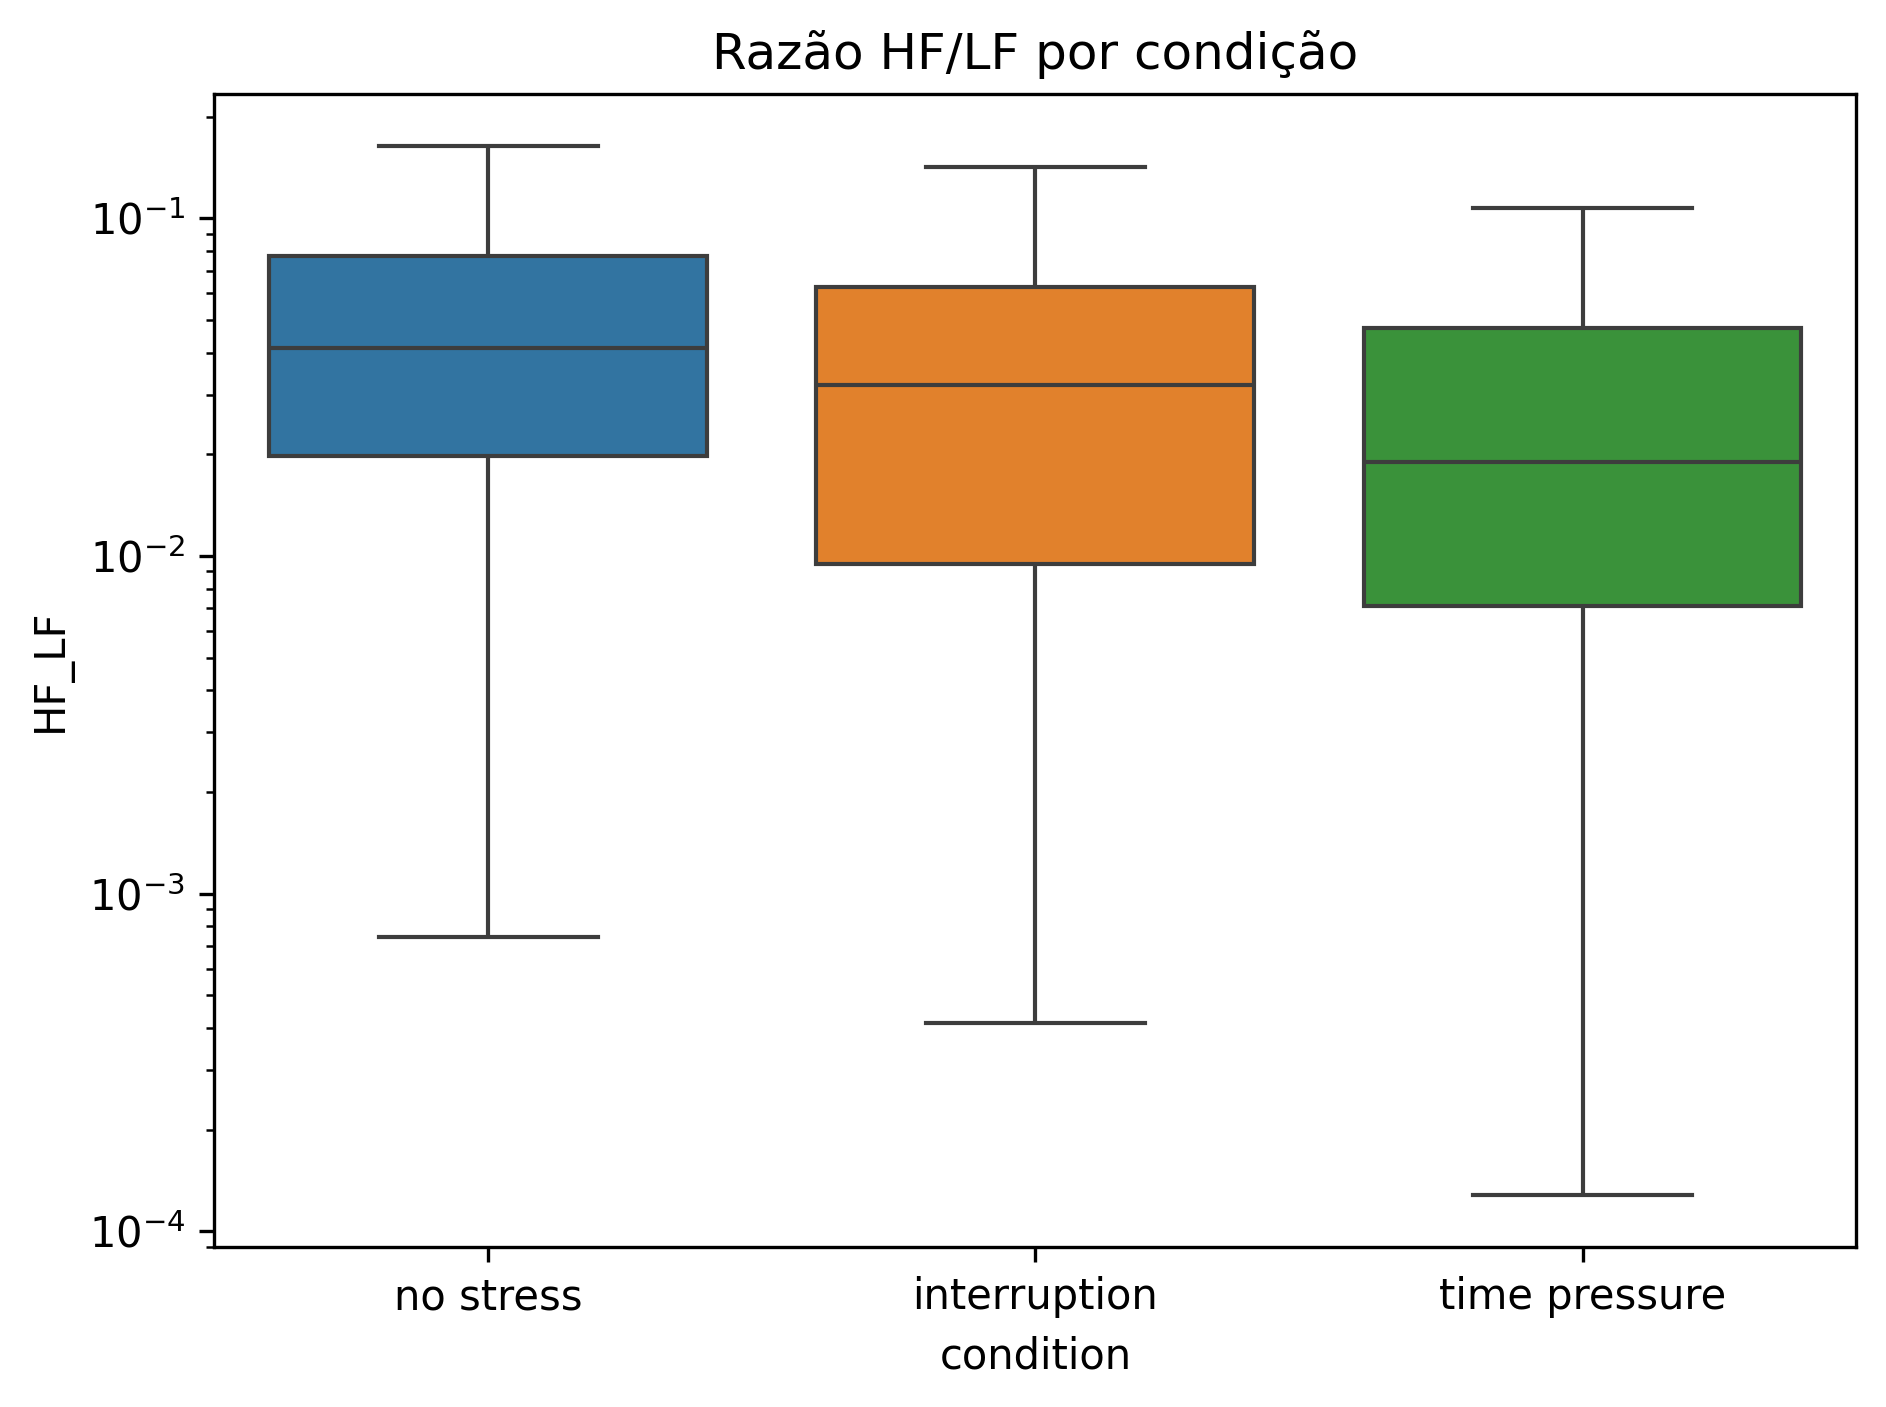
\includegraphics[width=0.8\linewidth]{../../../images/Anderson/box_hf_lf_condition_logscale.png}
    \caption{Boxplot HF/LF por condição.}
    \label{fig:hflf_box}
\end{figure}

É importante lembrar que, embora HF represente predominantemente a atividade parassimpática e LF inclua componentes simpáticos e barorreflexos, a razão LF/HF deve ser interpretada com cautela, servindo apenas como indicador relativo de deslocamento do balanço autonômico.

\subsubsection{Potência total e distribuição espectral}

Entre os índices de potência, a variável \textit{TP} (total power) representa a energia global da variabilidade dos intervalos RR, enquanto \textit{VLF\_PCT} descreve a contribuição relativa das oscilações de muito baixa frequência \cite{R3}. 

Na Figura~\ref{fig:BXP_TP_VLFPCT} observa-se que a potência total (\textit{TP}) apresentou valores ligeiramente mais altos sob \textit{time pressure}. 
Embora a literatura clássica reporte reduções de \textit{TP} e \textit{HF} em estresse agudo \cite{R1}, este comportamento divergente pode indicar particularidades do conjunto de dados e da segmentação dos sinais, não necessariamente uma inconsistência fisiológica. 

Assim como, \textit{VLF\_PCT} mostrou valores ligeiramente mais altos nessa condição, sugerindo maior participação relativa dos componentes de muito baixa frequência (Figura~\ref{fig:BXP_TP_VLFPCT}).

\begin{figure}[H]
    \centering
    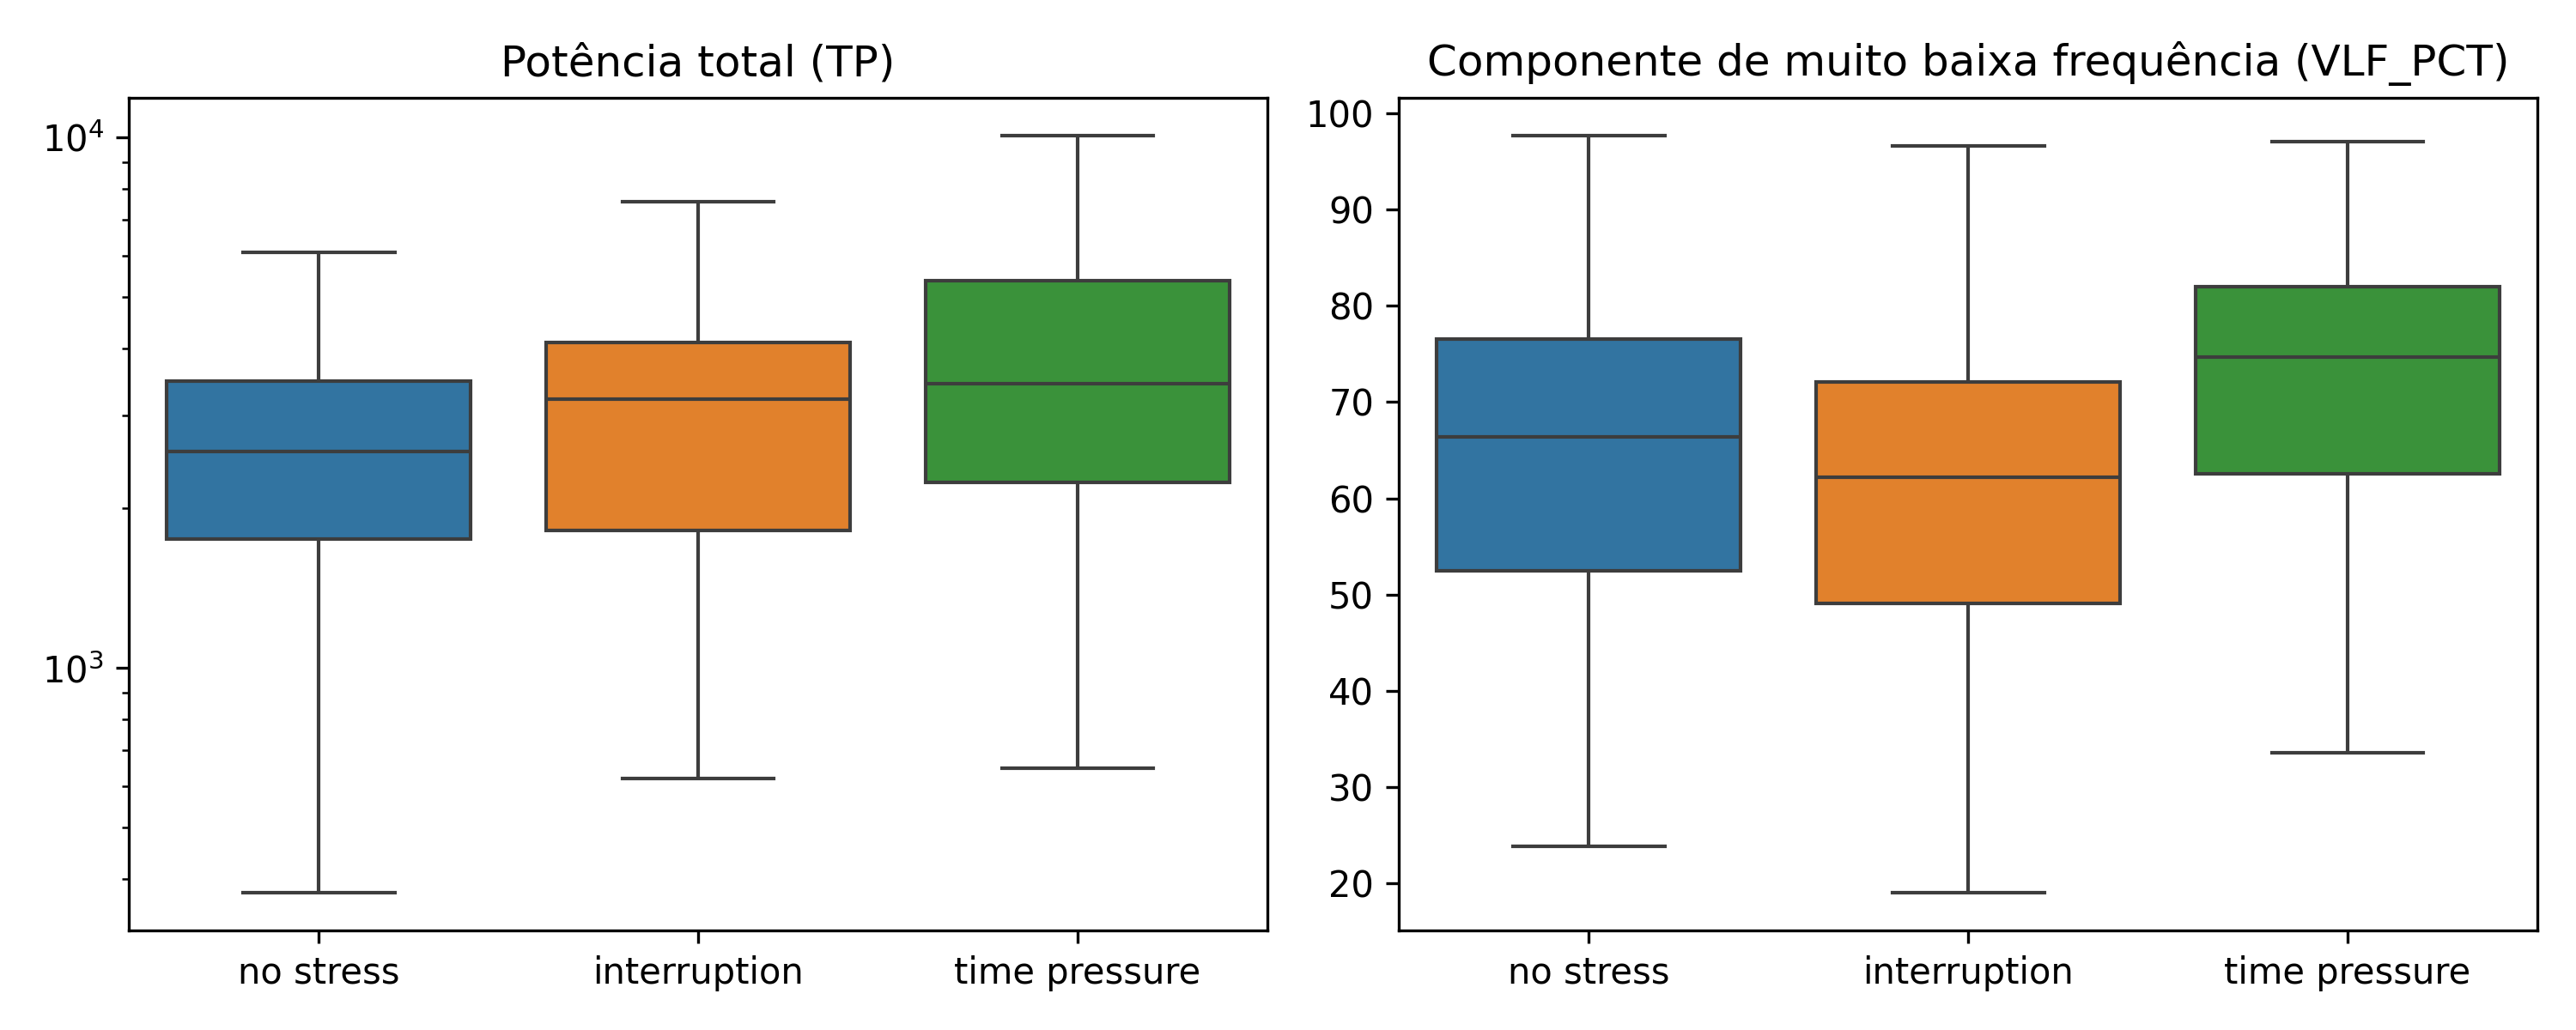
\includegraphics[width=\linewidth]{../../../images/Anderson/box_tp_vlfpct_condition.png}
    \caption{Boxplots por condição: \textit{TP}, \textit{VLF\_PCT}}
    \label{fig:BXP_TP_VLFPCT}
\end{figure}

Essas variações, embora sutis, indicam que a resposta ao aumento de demanda não se limitou à redistribuição entre bandas (LF e HF), mas também envolveu alterações na potência total do espectro.

\subsection{Redundância e seleção}

Vários dos preditores calculados apresentam definições semelhantes ou alto grau de correlação mútua. Por exemplo, RMSSD e pNN50 ambos quantificam variabilidade de curto prazo dominada pelo sistema parassimpático (vagal) e, como previsto, mostraram-se fortemente correlacionados entre si nos dados ($r \approx 0.79$). O que já era conhecido, tanto que RMSSD é frequentemente preferido ao pNN50 por ter propriedades estatísticas mais estáveis \cite{R3}. 

Essa redundância sugere que nem todos os preditores fornecem informação inédita para o modelo de regressão ou de classificação. Sabendo disso e das informações anteriores, escolhemos o subconjunto de preditores formado por 

(i) \textbf{Cronotropia} (\textit{HR}, \textit{MEDIAN\_RR}); 

(ii) \textbf{Variabilidade de curto prazo vagal} (\textit{RMSSD}, \textit{SDSD\_REL\_RR}); 

(iii) \textbf{Dispersão global de longo prazo} (\textit{SD2}, \textit{SDRR\_REL\_RR}); 

(iv) \textbf{Componentes espectrais} (\textit{LF}, \textit{HF}, \textit{VLF\_PCT}, \textit{TP}); e 

(v) a \textbf{Razão espectral inversa} (\textit{HF\_LF}).

Métricas não lineares, como a entropia amostral (Sampen), foram calculadas mas não mostraram poder discriminativo relevante.

\subsection{Análise de Componentes Principais (PCA) e Biplot}
O PCA aplicado aos 12 preditores padronizados explicou cerca de \textbf{71,2\%} da variância total nas duas primeiras componentes (\textit{PC1} = 40,5\%, \textit{PC2} = 30,7\%). 
O mapa \textit{PC1}$\times$\textit{PC2} exibiu sobreposição entre classes, mas com tendência ordenada: registros de \textit{time pressure} concentraram-se na região associada a \textit{HR} mais alta e \textit{MEDIAN\_RR} menor, enquanto \textit{no stress} ocupou o quadrante oposto, coerente com maior modulação vagal. 

A \textit{PC1} representou o eixo de controle cardíaco (com \textit{HR} e \textit{MEDIAN\_RR}), enquanto a \textit{PC2} refletiu diferenças de potência espectral (\textit{HF}, \textit{LF}, \textit{TP}). 
No \textit{biplot} (Figura~\ref{fig:biplot_pca}), as cargas (\textit{loadings}) reforçam essa separação: \textit{HR} e \textit{MEDIAN\_RR} mostram orientação oposta, confirmando correlação negativa, e as variáveis \textit{HF} e \textit{HF\_LF} agrupam-se, indicando captação conjunta do componente vagal.  

Em geral, como apresentado na Figura \ref{fig:biplot_pca}, o \textit{biplot} evidencia um eixo principal associado à frequência cardíaca e outro à variação espectral, reproduzindo o padrão fisiológico esperado e mostrando que as condições se distribuem de forma contínua ao longo do espectro autonômico.

\begin{figure}[H]
    \centering
    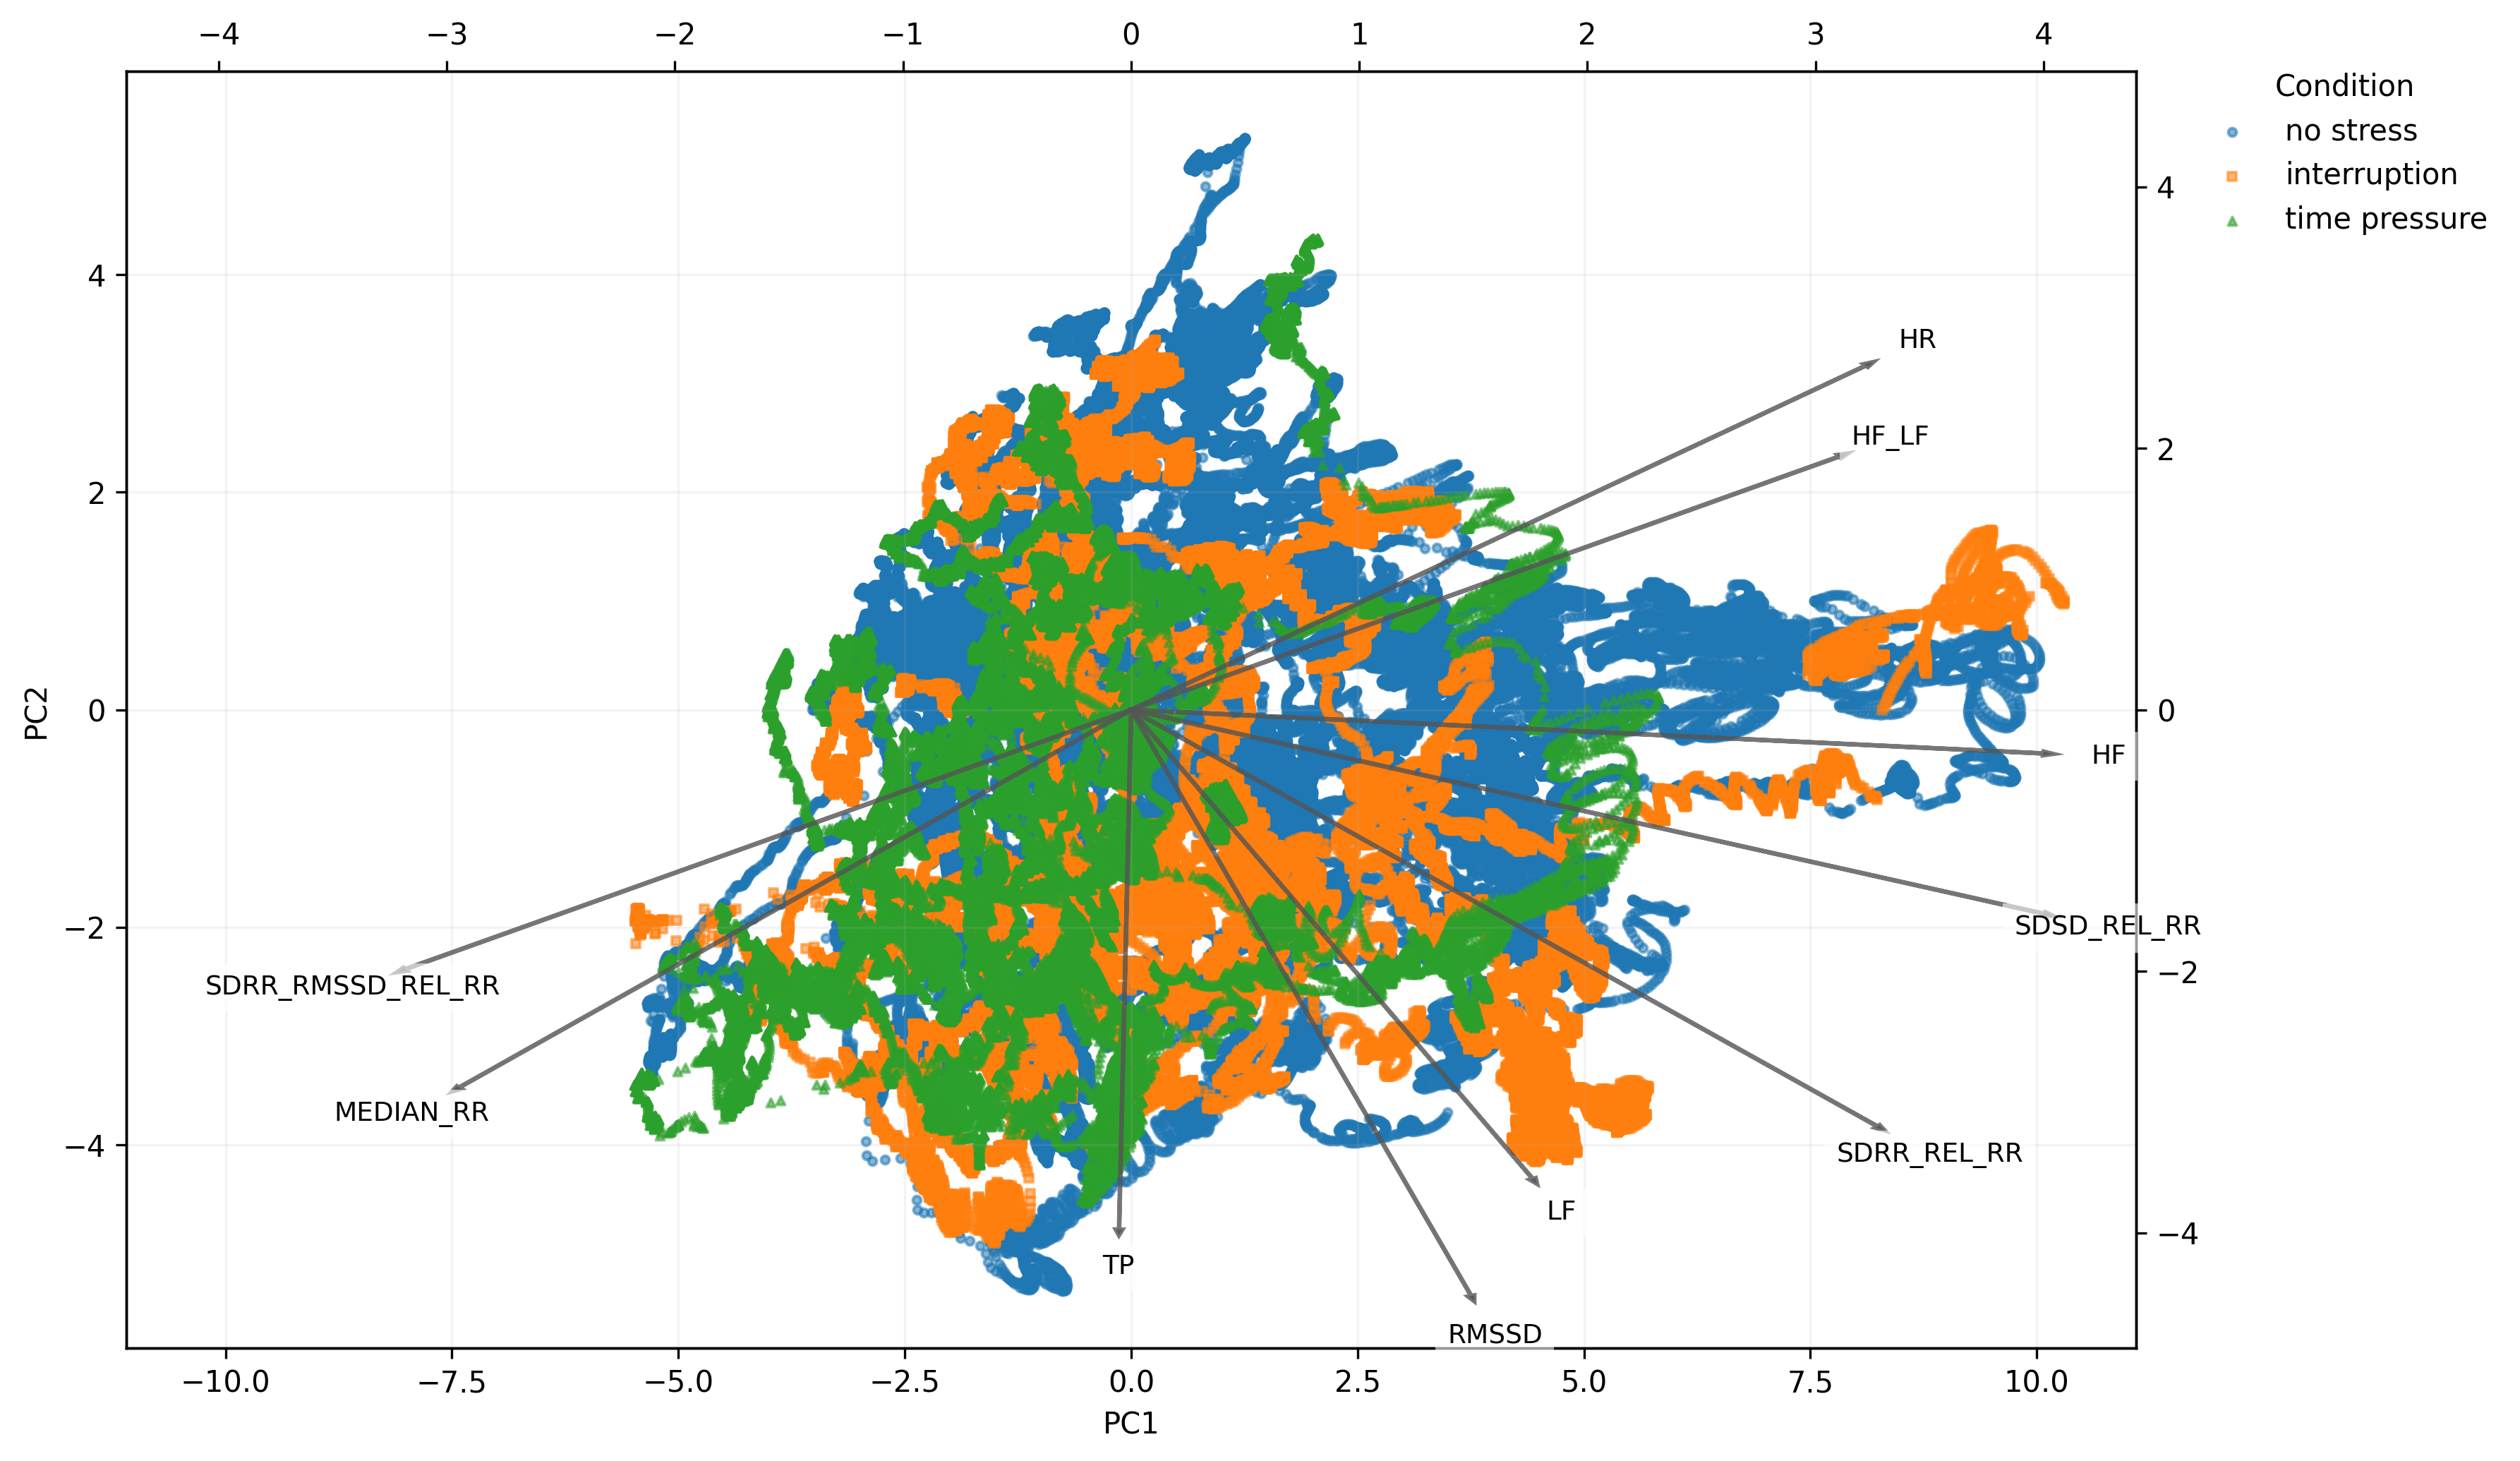
\includegraphics[width=\linewidth]{../../../images/Anderson/biplot_pca_2variaveis.png}
    \caption{Biplot das duas primeiras componentes principais (PC1 e PC2) obtidas a partir dos 12 preditores padronizados.}
    \label{fig:biplot_pca}
\end{figure}


\section{Conclusão}

Em conclusão, a explicação e discussão crítica dos resultados do pré-processamento reforçam que os dados estão consistentes com os princípios da fisiologia cardíaca. O pré-processamento, incluindo padronização e eliminação de variáveis altamente correlacionadas, preservou a diversidade fisiológica entre métricas cronotrópicas, temporais e espectrais. Dessa forma, conseguimos enriquecer a análise exploratória com contexto biológico, oferecendo ao leitor uma compreensão mais profunda de como os resultados do pré-processamento se conectam à realidade fisiológica subjacente aos dados.

\section*{Acknowledgment}

The preferred spelling of the word ``acknowledgment'' in America is without 
an ``e'' after the ``g''. Avoid the stilted expression ``one of us (R. B. 
G.) thanks $\ldots$''. Instead, try ``R. B. G. thanks$\ldots$''. Put sponsor 
acknowledgments in the unnumbered footnote on the first page.

\section*{References}

\begin{thebibliography}{00}
\bibitem{R1} R. Shaffer and J. P. Ginsberg, “An Overview of Heart Rate Variability Metrics and Norms,” Frontiers in Public Health, vol. 5, p. 258, Apr. 2017. [Online]. Available: https://pmc.ncbi.nlm.nih.gov/articles/PMC5900369/
\bibitem{R2} American Heart Association, “Tachycardia (Fast Heart Rate),” Heart.org, 2024. [Online]. Available: https://www.heart.org/en/health-topics/arrhythmia/about-arrhythmia/tachycardia--fast-heart-rate.
\bibitem{R3} Task Force of the European Society of Cardiology and the North American Society of Pacing and Electrophysiology, “Heart rate variability: Standards of measurement, physiological interpretation and clinical use,” Circulation, vol. 93, no. 5, pp. 1043–1065, 1996. [Online]. Available: https://www.escardio.org/static-file/Escardio/Guidelines/Scientific-Statements/guidelines-Heart-Rate-Variability-FT-1996.pdf
\end{thebibliography}

\vspace{12pt}
\color{red}
IEEE conference templates contain guidance text for composing and formatting conference papers. Please ensure that all template text is removed from your conference paper prior to submission to the conference. Failure to remove the template text from your paper may result in your paper not being published.

\end{document}
